\documentclass{standalone}
\usepackage{tikz}
\usetikzlibrary{patterns, positioning}


\begin{document}
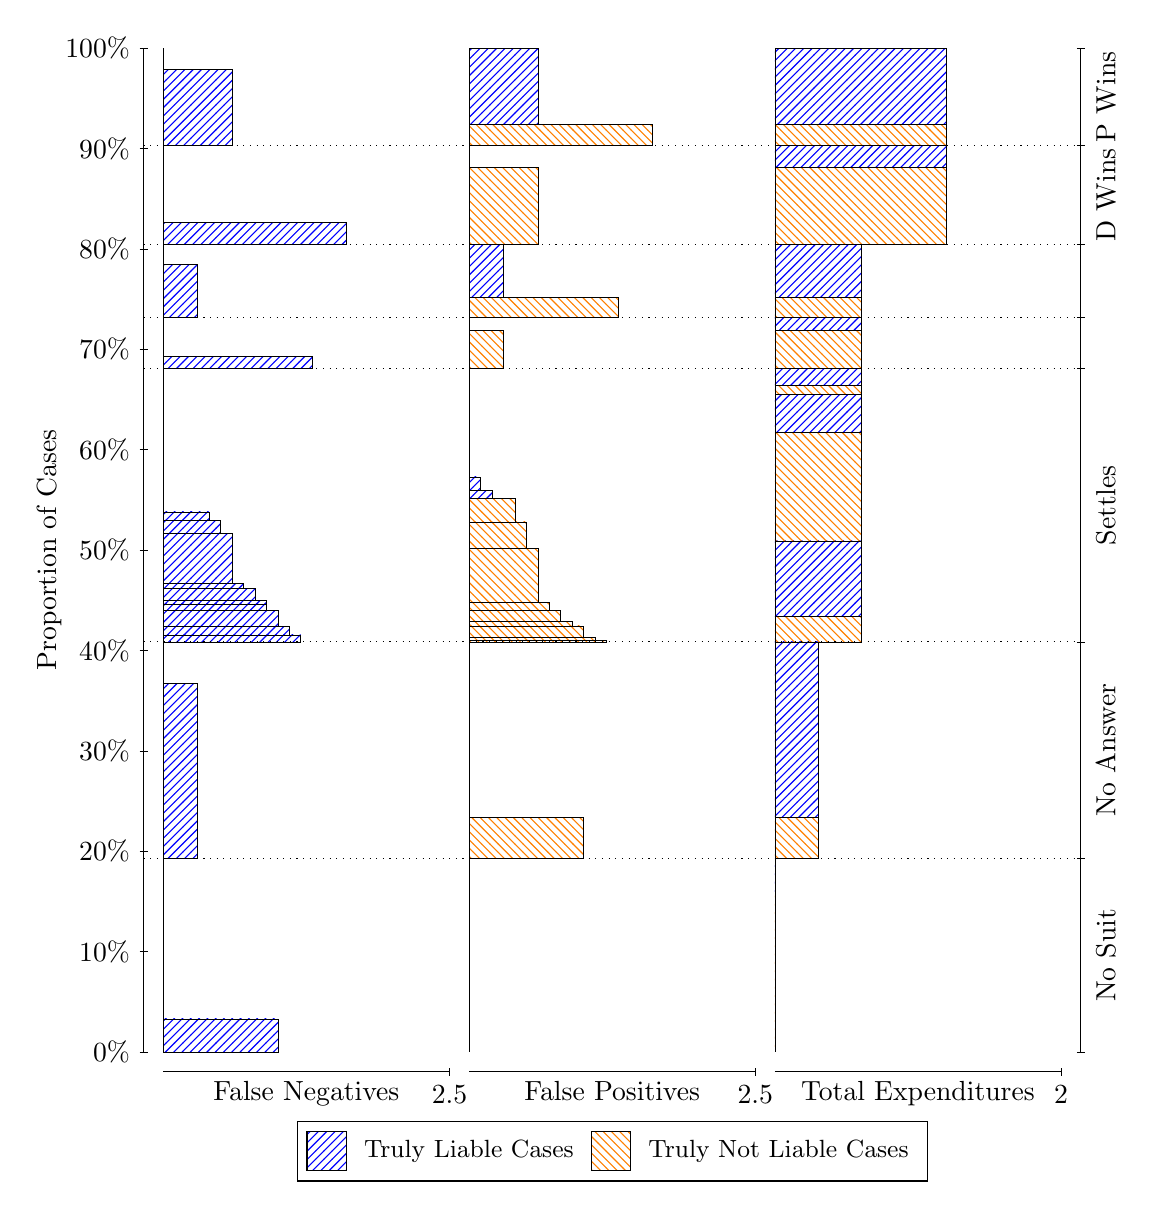
\begin{tikzpicture}
\draw[black, very thin] (1.5,1.75) -- (1.5,14.5);
\node[rotate=90, text=black, anchor=center] at (0.3, 8.125) {Proportion of Cases};
\draw[black, very thin] (1.45,1.75) -- (1.55,1.75);
\node[text=black, anchor=east] at (1.45, 1.75) {0\%};
\draw[black, very thin] (1.45,3.025) -- (1.55,3.025);
\node[text=black, anchor=east] at (1.45, 3.025) {10\%};
\draw[black, very thin] (1.45,4.3) -- (1.55,4.3);
\node[text=black, anchor=east] at (1.45, 4.3) {20\%};
\draw[black, very thin] (1.45,5.575) -- (1.55,5.575);
\node[text=black, anchor=east] at (1.45, 5.575) {30\%};
\draw[black, very thin] (1.45,6.85) -- (1.55,6.85);
\node[text=black, anchor=east] at (1.45, 6.85) {40\%};
\draw[black, very thin] (1.45,8.125) -- (1.55,8.125);
\node[text=black, anchor=east] at (1.45, 8.125) {50\%};
\draw[black, very thin] (1.45,9.4) -- (1.55,9.4);
\node[text=black, anchor=east] at (1.45, 9.4) {60\%};
\draw[black, very thin] (1.45,10.675) -- (1.55,10.675);
\node[text=black, anchor=east] at (1.45, 10.675) {70\%};
\draw[black, very thin] (1.45,11.95) -- (1.55,11.95);
\node[text=black, anchor=east] at (1.45, 11.95) {80\%};
\draw[black, very thin] (1.45,13.225) -- (1.55,13.225);
\node[text=black, anchor=east] at (1.45, 13.225) {90\%};
\draw[black, very thin] (1.45,14.5) -- (1.55,14.5);
\node[text=black, anchor=east] at (1.45, 14.5) {100\%};

\draw[black, very thin] (13.4,1.75) -- (13.4,14.5);
\draw[black, very thin] (13.35,1.75) -- (13.45,1.75);
\node[anchor=west] at (13.35, 1.75) {};
\draw[black, very thin] (13.35,4.2043) -- (13.45,4.2043);
\node[anchor=west] at (13.35, 4.2043) {};
\draw[black, very thin] (13.35,6.9584) -- (13.45,6.9584);
\node[anchor=west] at (13.35, 6.9584) {};
\draw[black, very thin] (13.35,10.427) -- (13.45,10.427);
\node[anchor=west] at (13.35, 10.427) {};
\draw[black, very thin] (13.35,11.076) -- (13.45,11.076);
\node[anchor=west] at (13.35, 11.076) {};
\draw[black, very thin] (13.35,12.007) -- (13.45,12.007);
\node[anchor=west] at (13.35, 12.007) {};
\draw[black, very thin] (13.35,13.26) -- (13.45,13.26);
\node[anchor=west] at (13.35, 13.26) {};
\draw[black, very thin] (13.35,14.5) -- (13.45,14.5);
\node[anchor=west] at (13.35, 14.5) {};

\draw[black, very thin, pattern color=blue, pattern=north east lines] (1.75,1.75) rectangle (3.2033,2.1697);
\draw[black, very thin, pattern color=orange, pattern=north west lines] (1.75,2.1697) rectangle (1.75,4.2043);
\draw[black, very thin, pattern color=blue, pattern=north east lines] (1.75,4.2043) rectangle (2.186,6.4336);
\draw[black, very thin, pattern color=orange, pattern=north west lines] (1.75,6.4336) rectangle (1.75,6.9584);
\draw[black, very thin, pattern color=blue, pattern=north east lines] (1.75,6.9584) rectangle (3.494,7.0465);
\draw[black, very thin, pattern color=blue, pattern=north east lines] (1.75,7.0465) rectangle (3.3487,7.154);
\draw[black, very thin, pattern color=blue, pattern=north east lines] (1.75,7.154) rectangle (3.2033,7.36);
\draw[black, very thin, pattern color=blue, pattern=north east lines] (1.75,7.36) rectangle (3.058,7.4408);
\draw[black, very thin, pattern color=blue, pattern=north east lines] (1.75,7.4408) rectangle (3.058,7.4824);
\draw[black, very thin, pattern color=blue, pattern=north east lines] (1.75,7.4824) rectangle (2.9127,7.642);
\draw[black, very thin, pattern color=blue, pattern=north east lines] (1.75,7.642) rectangle (2.7673,7.7044);
\draw[black, very thin, pattern color=blue, pattern=north east lines] (1.75,7.7044) rectangle (2.622,8.3317);
\draw[black, very thin, pattern color=blue, pattern=north east lines] (1.75,8.3317) rectangle (2.4767,8.5035);
\draw[black, very thin, pattern color=blue, pattern=north east lines] (1.75,8.5035) rectangle (2.3313,8.6086);
\draw[black, very thin, pattern color=orange, pattern=north west lines] (1.75,8.6086) rectangle (1.75,10.427);
\draw[black, very thin, pattern color=blue, pattern=north east lines] (1.75,10.427) rectangle (3.6393,10.588);
\draw[black, very thin, pattern color=orange, pattern=north west lines] (1.75,10.588) rectangle (1.75,11.076);
\draw[black, very thin, pattern color=blue, pattern=north east lines] (1.75,11.076) rectangle (2.186,11.75);
\draw[black, very thin, pattern color=orange, pattern=north west lines] (1.75,11.75) rectangle (1.75,12.007);
\draw[black, very thin, pattern color=blue, pattern=north east lines] (1.75,12.007) rectangle (4.0753,12.282);
\draw[black, very thin, pattern color=orange, pattern=north west lines] (1.75,12.282) rectangle (1.75,13.26);
\draw[black, very thin, pattern color=blue, pattern=north east lines] (1.75,13.26) rectangle (2.622,14.226);
\draw[black, very thin, pattern color=orange, pattern=north west lines] (1.75,14.226) rectangle (1.75,14.5);
\draw[black, very thin, pattern color=orange, pattern=north west lines] (5.6333,1.75) rectangle (5.6333,3.7846);
\draw[black, very thin, pattern color=blue, pattern=north east lines] (5.6333,3.7846) rectangle (5.6333,4.2043);
\draw[black, very thin, pattern color=orange, pattern=north west lines] (5.6333,4.2043) rectangle (7.0867,4.7291);
\draw[black, very thin, pattern color=blue, pattern=north east lines] (5.6333,4.7291) rectangle (5.6333,6.9584);
\draw[black, very thin, pattern color=orange, pattern=north west lines] (5.6333,6.9584) rectangle (7.3773,6.9796);
\draw[black, very thin, pattern color=orange, pattern=north west lines] (5.6333,6.9796) rectangle (7.232,7.0186);
\draw[black, very thin, pattern color=orange, pattern=north west lines] (5.6333,7.0186) rectangle (7.0867,7.1619);
\draw[black, very thin, pattern color=orange, pattern=north west lines] (5.6333,7.1619) rectangle (6.9413,7.2185);
\draw[black, very thin, pattern color=orange, pattern=north west lines] (5.6333,7.2185) rectangle (6.796,7.3594);
\draw[black, very thin, pattern color=orange, pattern=north west lines] (5.6333,7.3594) rectangle (6.6507,7.4632);
\draw[black, very thin, pattern color=orange, pattern=north west lines] (5.6333,7.4632) rectangle (6.5053,8.1426);
\draw[black, very thin, pattern color=orange, pattern=north west lines] (5.6333,8.1426) rectangle (6.36,8.4818);
\draw[black, very thin, pattern color=orange, pattern=north west lines] (5.6333,8.4818) rectangle (6.2147,8.7771);
\draw[black, very thin, pattern color=blue, pattern=north east lines] (5.6333,8.7771) rectangle (5.924,8.8822);
\draw[black, very thin, pattern color=blue, pattern=north east lines] (5.6333,8.8822) rectangle (5.7787,9.054);
\draw[black, very thin, pattern color=blue, pattern=north east lines] (5.6333,9.054) rectangle (5.6333,10.427);
\draw[black, very thin, pattern color=orange, pattern=north west lines] (5.6333,10.427) rectangle (6.0693,10.915);
\draw[black, very thin, pattern color=blue, pattern=north east lines] (5.6333,10.915) rectangle (5.6333,11.076);
\draw[black, very thin, pattern color=orange, pattern=north west lines] (5.6333,11.076) rectangle (7.5227,11.333);
\draw[black, very thin, pattern color=blue, pattern=north east lines] (5.6333,11.333) rectangle (6.0693,12.007);
\draw[black, very thin, pattern color=orange, pattern=north west lines] (5.6333,12.007) rectangle (6.5053,12.985);
\draw[black, very thin, pattern color=blue, pattern=north east lines] (5.6333,12.985) rectangle (5.6333,13.26);
\draw[black, very thin, pattern color=orange, pattern=north west lines] (5.6333,13.26) rectangle (7.9587,13.534);
\draw[black, very thin, pattern color=blue, pattern=north east lines] (5.6333,13.534) rectangle (6.5053,14.5);
\draw[black, very thin, pattern color=orange, pattern=north west lines] (9.5167,1.75) rectangle (9.5167,3.7846);
\draw[black, very thin, pattern color=blue, pattern=north east lines] (9.5167,3.7846) rectangle (9.5167,4.2043);
\draw[black, very thin, pattern color=orange, pattern=north west lines] (9.5167,4.2043) rectangle (10.062,4.7291);
\draw[black, very thin, pattern color=blue, pattern=north east lines] (9.5167,4.7291) rectangle (10.062,6.9584);
\draw[black, very thin, pattern color=orange, pattern=north west lines] (9.5167,6.9584) rectangle (10.607,7.2816);
\draw[black, very thin, pattern color=blue, pattern=north east lines] (9.5167,7.2816) rectangle (10.607,8.2403);
\draw[black, very thin, pattern color=orange, pattern=north west lines] (9.5167,8.2403) rectangle (10.607,9.6198);
\draw[black, very thin, pattern color=blue, pattern=north east lines] (9.5167,9.6198) rectangle (10.607,10.102);
\draw[black, very thin, pattern color=orange, pattern=north west lines] (9.5167,10.102) rectangle (10.607,10.218);
\draw[black, very thin, pattern color=blue, pattern=north east lines] (9.5167,10.218) rectangle (10.607,10.427);
\draw[black, very thin, pattern color=orange, pattern=north west lines] (9.5167,10.427) rectangle (10.607,10.915);
\draw[black, very thin, pattern color=blue, pattern=north east lines] (9.5167,10.915) rectangle (10.607,11.076);
\draw[black, very thin, pattern color=orange, pattern=north west lines] (9.5167,11.076) rectangle (10.607,11.333);
\draw[black, very thin, pattern color=blue, pattern=north east lines] (9.5167,11.333) rectangle (10.607,12.007);
\draw[black, very thin, pattern color=orange, pattern=north west lines] (9.5167,12.007) rectangle (11.697,12.985);
\draw[black, very thin, pattern color=blue, pattern=north east lines] (9.5167,12.985) rectangle (11.697,13.26);
\draw[black, very thin, pattern color=orange, pattern=north west lines] (9.5167,13.26) rectangle (11.697,13.534);
\draw[black, very thin, pattern color=blue, pattern=north east lines] (9.5167,13.534) rectangle (11.697,14.5);
\draw[black, dotted] (1.5,4.2043) -- (13.4,4.2043);
\draw[black, dotted] (1.5,6.9584) -- (13.4,6.9584);
\draw[black, dotted] (1.5,10.427) -- (13.4,10.427);
\draw[black, dotted] (1.5,11.076) -- (13.4,11.076);
\draw[black, dotted] (1.5,12.007) -- (13.4,12.007);
\draw[black, dotted] (1.5,13.26) -- (13.4,13.26);
\draw[black, very thin] (1.75,1.5) -- (5.3833,1.5);
\node[text=black, anchor=north] at (3.5667, 1.5) {False Negatives};
\draw[black, very thin] (5.3833,1.45) -- (5.3833,1.55);
\node[text=black, anchor=north] at (5.3833, 1.45) {2.5};

\draw[black, very thin] (5.6333,1.5) -- (9.2667,1.5);
\node[text=black, anchor=north] at (7.45, 1.5) {False Positives};
\draw[black, very thin] (9.2667,1.45) -- (9.2667,1.55);
\node[text=black, anchor=north] at (9.2667, 1.45) {2.5};

\draw[black, very thin] (9.5167,1.5) -- (13.15,1.5);
\node[text=black, anchor=north] at (11.333, 1.5) {Total Expenditures};
\draw[black, very thin] (13.15,1.45) -- (13.15,1.55);
\node[text=black, anchor=north] at (13.15, 1.45) {2};

\node[text=black, centered, rotate=90] at (13.72, 2.9771) {No Suit};
\node[text=black, centered, rotate=90] at (13.72, 5.5813) {No Answer};
\node[text=black, centered, rotate=90] at (13.72, 8.6929) {Settles};


\node[text=black, centered, rotate=90] at (13.72, 12.633) {D Wins};
\node[text=black, centered, rotate=90] at (13.72, 13.88) {P Wins};

\draw (7.449999999999999,1.5) node[draw=none] (baseCoordinate) {};
\begin{scope}[align=center]
        \matrix[scale=0.5, draw=black, below=0.5cm of baseCoordinate, nodes={draw}, column sep=0.1cm]{
            \node[rectangle, draw, minimum width=0.5cm, minimum height=0.5cm, pattern color=blue, pattern=north east lines] {}; &
            \node[draw=none, font=\small, text=black] (B) {Truly Liable Cases}; &
            \node[rectangle, draw, minimum width=0.5cm, minimum height=0.5cm, pattern color=orange, pattern=north west lines] {}; &
            \node[draw=none, font=\small, text=black] (B) {Truly Not Liable Cases}; \\
            };
\end{scope}

\end{tikzpicture}
\end{document}